%
% Bachelor Thesis
% Sven Hodapp
%


% -----------
% 1. Präambel
% -----------


% Allgemeine Einstellungen
% ------------------------
\documentclass[
	pdftex,%              PDFTex verwenden da wir ausschliesslich ein PDF erzeugen.
	a4paper,%             Wir verwenden A4 Papier.
	oneside,%             Einseitiger Druck.
	12pt,%                Grosse Schrift, besser geeignet für A4.
	halfparskip,%         Halbe Zeile Abstand zwischen Absätzen.
	%chapterprefix,%       Kapitel mit 'Kapitel' anschreiben.
	headsepline,%         Linie nach Kopfzeile.
	footsepline,%         Linie vor Fusszeile.
	bibtotocnumbered,%    Literaturverzeichnis im Inhaltsverzeichnis nummeriert einfügen.
	idxtotoc%             Index ins Inhaltsverzeichnis einfügen.
]{article}

\usepackage[utf8]{inputenc}
\usepackage[german]{babel}   % deutsche Silbentrennung
\selectlanguage{german}   % damit Table Of Contents Inhaltsverzeichnis genannt wird

\usepackage{geometry}   % Seitenränder einstellbar
\usepackage{textcomp}   % Sonderzeichen, wie Eurosymbol
\usepackage[hyphens]{url} % URLs korrekt umbrechen.



% Bilder, Farben, farbige Tabellen
% --------------------------------
\usepackage{graphicx, color, colortbl}
\usepackage[svgnames]{xcolor} % Required to specify font color
\usepackage{longtable}
\usepackage{lscape}
\usepackage{array}       % Erweiterte Tabelleneigenschaften.
%\usepackage{floatflt}   % Bild kann von Text umflossen werden.



% Palatino Schrift
% ----------------
%\usepackage[T1]{fontenc}
%\usepackage[osf]{mathpazo}   % osf aktiviert Mediävalziffern/Minuskelziffern



% Syntax-Highlighting
% -------------------
% Src: http://tihlde.org/~eivindw/latex-listings-for-scala/
\definecolor{dkgreen}{rgb}{0,0.6,0}
\definecolor{gray}{rgb}{0.5,0.5,0.5}
\definecolor{mauve}{rgb}{0.58,0,0.82}

\usepackage{listings}

% "define" Scala
\lstdefinelanguage{Scala}{
  morekeywords={abstract,case,catch,class,def,%
    do,else,extends,false,final,finally,%
    for,if,implicit,import,match,mixin,%
    new,null,object,override,package,%
    private,protected,requires,return,sealed,%
    super,this,throw,trait,true,try,%
    type,val,var,while,with,yield},
  otherkeywords={=>,<-,<\%,<:,>:,\#,@},
  sensitive=true,
  morecomment=[l]{//},
  morecomment=[n]{/*}{*/},
  morestring=[b]",
  morestring=[b]',
  morestring=[b]"""
}

% src: http://lenaherrmann.net/2010/05/20/
%      javascript-syntax-highlighting-in-the-latex-listings-package
\lstdefinelanguage{JavaScript}{
  keywords={
    typeof, new, true, false, catch, function, return, null,
    catch, switch, var, if, in, while, do, else, case, break
  },
  ndkeywords={class, export, boolean, throw, implements, import, this},
  sensitive=false,
  comment=[l]{//},
  morecomment=[s]{/*}{*/},
  morestring=[b]',
  morestring=[b]"
}

\lstset{
  frame=tb,
  language=bash,
  aboveskip=3mm,
  belowskip=3mm,
  showstringspaces=false,
  columns=flexible,
  basicstyle={\fontsize{10}{11}\ttfamily},
  numbers=left,
  numberstyle=\tiny\color{gray},
  keywordstyle=\color{blue},
  commentstyle=\color{dkgreen},
  stringstyle=\color{mauve},
  frame=single,
  breaklines=true,
  breakatwhitespace=true,
  tabsize=2,
  extendedchars=\true,
  inputencoding=utf8,
  escapeinside={\%*}{*)}  % http://tex.stackexchange.com/questions/24528/
}


% Sonstige Pakete
% ---------------
%\usepackage{anysize}   % Seitenränder verändern
%\usepackage{setspace}   % 1.5em Zeilenabstand \begin{onehalfspacing}
\usepackage{bibgerm}   % Anzeigestil des Literaturverzeichnis (gerabbrv)
\usepackage{paralist}  % Individualisierte Aufzählungen


% Global Variables
% ----------------

\newcommand{\thema}{Firewall unter Debian 6.0 Squeeze}
\newcommand{\untertitel}{Mit iptables in einer DMZ-Umgebung}
\newcommand{\schlagworte}{iptables, firewalls, dmz, security, linux, debian}
\newcommand{\autor}{Marc Bumiller, Sven Hodapp}


% Title Page
% ----------
% (thanks to: http://www.latextemplates.com/template/minimalist-book-title-page)

\newcommand*{\plogo}{\fbox{$\mathcal{HTWG}$}} % Generic publisher logo

\newcommand*{\titleTH}{\begingroup % Create the command for including the title page in the document
\raggedleft % Right-align all text
\vspace*{\baselineskip} % Whitespace at the top of the page

{\Large \autor}\\[0.167\textheight] % Author name

{\LARGE\bfseries ITSEC: Laborbericht}\\[\baselineskip] % First part of the title, if it is unimportant consider making the font size smaller to accentuate the main title

{\textcolor{Red}{\Huge \thema}}\\[\baselineskip] % Main title which draws the focus of the reader

{\Large \textit{\untertitel}}\par % Tagline or further description

\vfill % Whitespace between the title block and the publisher

{\large Hochschule Konstanz \plogo}\par % Publisher and logo

\vspace*{3\baselineskip} % Whitespace at the bottom of the page
\endgroup}


% PDF Eigenschaften
% -----------------
\usepackage
[
	colorlinks=false,
	bookmarks = true,
	pdftitle={\thema},
	pdfauthor={\autor},
	pdfsubject={\untertitel},
	pdfkeywords={\schlagworte},
	urlcolor=blue,
	pdfstartview=FitH
]{hyperref}





% --------------------
% 2. Dokumenten Anfang
% --------------------

\begin{document}

\pagenumbering{roman}

% Deckblatt
% ---------

\pagestyle{empty}
\titleTH
\newpage



% Inhaltsverzeichnis anzeigen
% ---------------------------
\tableofcontents
\newpage

\pagenumbering{arabic}

% ---------
% 3. Inhalt
% ---------

\section{Einleitung}

Im Dezember 1970 wurde der Vorgänger des Internets, das ARPANET, offiziell
verabschiedet. Eine der ersten Applikationen war die E-Mail.
Am 1.1.1983 wurde ARPANET auf TCP/IP als Protokoll umgestellt,
da das vorherige Protokoll mit wachsender Größe des ARPANET Schwierigkeiten
bekam.

Neben ARPANET entwickelten sich noch zahlreiche andere Computernetzwerke,
aber das erfolgreichste war das aus dem akademischen Umfeld stammende NSFNET,
welches heute als Internet bezeichnet wird.

Damals war das Internet eine heile Welt, jeder vertraute jedem und Sicherheit
wurde zu dieser Zeit noch nicht groß geschrieben.
Das änderte sich jedoch im November 1988, als der Morris-Wurm sein unwesen
trieb, der förmlich eine Epidemie im Internet auslöste. Dies bewegte Firmen
dazu, sich Gedanken über den Schutz ihrer Netzwerke zu machen.

Die ersten Firewallsysteme wurden bei DEC bzw. AT\&T entwickelt. Dabei handelte
es sich um einen Gatekeeper, der als einziger Zugriff auf das Internet hatte
und somit den Zugang zu diesem kontrollierte und ein Gate welches den Zugriff
vom internen Netzwerk auf den Gatekeeper als Paketfilter überwachte.
1991 wurde die erste kommerizielle Firewall \emph{DEC-SEAL} verkauft.\cite{iptables}

\paragraph{Heutige Firewalls} bestehen meist aus einer Kombination aus
Paketfilter und Proxy. Falls der Datendurchsatz in einem System sehr
hoch ist, werden oft reine Paketfilter eingesetzt.\cite{iptables}


\subsection{Firewall-Technologien}\label{sec.fw-tec}

\paragraph{Zustandslose Paketfilter} ist die einfachste Technologie und
wurde bereits 1989 von Jeffrey C. Mogul als {\tt screend} implementiert.
Ein Paketfilter agiert dabei wie ein intelligenter Router, der
neben der Paketweiterleitung auch entscheidet ob ein Paket
weitergeleitet werden darf oder verworfen werden soll.
Ein IP-Paketfiler analysiert somit den IP-Paketheader.
Ein vom Administrator vorgegebenes Regelwerk schreibt die Aktionen
des Filters vor. Da es zustandslos ist, wird jedes Paket für sich
betrachtet und darauf die Regeln angewandt.\cite{iptables}

\paragraph{Zustandsorientierte Paketfilter} Ab 1993 kamen die ersten
zustandsorientierten Paketfilter auf. Hier merkt sich die Firewall
ein- und ausgegangene Verbindungen und kann somit auch Entscheidungen
basierend auf den vergangenen Pakettransaktionen ausführen.
Die im Rahmen dieses Labors verwendete Software {\tt iptables} gehört zu dieser
Kategorie.\cite{iptables}

\paragraph{Curcuit Relay} ist ein Proxy, welcher auf der Transport-Schicht
sitzt.

\paragraph{Application-Level-Gateway} ist ein Proxy, der auf der Schicht
des Applikationsprotokolls arbeitet, d.h. dieser Proxy ist an ein einziges
spezielles Protokoll gebunden. Im schlimmsten Fall muss also für jede
Anwendung ein eigener Firewall-Proxy bereitgestellt werden.
Ein solcher Proxy kann eine sehr genaue Inspektion der mit dem jeweiligen
Protokoll verschickten Daten durchführen.\cite{iptables}

\paragraph{NAT}
Unter den Begriff \emph{Network Address Translation} fallen alle Verfahren,
welche Adressinformationen in Datenpaketen durch andere ersetzen.
Typischer Einsatzort sind beispielsweise Router, bei denen NAT nötig wird,
wenn ein LAN aus dem Internet nur über eine IP-Adresse sichtbar ist.
Kurz gesagt ermöglich es, dass viele Rechner unter der selben IP-Adresse auf Dienste
im Internet zugreifen.\cite{iptables}

\paragraph{DNAT}
\emph{Destination-NAT} verändert die Ziel-Adresse eines Pakets.
Neben der Ziel-IP im IP-Header kann auch der Ziel-Port in einem
TCP- bzw. UDP-Header geändert werden.
Eingesetzt wird das Verfahren um Pakete, welche an der öf\-fent\-lichen Adresse
des Routers eingehen, an einen anderen Rechner im LAN mit privater IP-Adresse
weiterzuleiten.

\paragraph{SNAT}
Möchte man statt der Ziel-Adresse die Quell-Adresse eines Pakets ändern, wird
dies als \emph{Source-NAT} bezeichnet.
Auch hier lässt sich logischerweise IP-Adresse und TCP- bzw. UDP-Port
modifzieren.
Dieses Verfahren wird nun nicht bei den eingehenden, sondern bei den ausgehenden
Paketen angewandt, um die private lokale Adresse durch die öffentliche zu
ersetzen.

\paragraph{Masquerading}
\emph{Masquerading} stellt eine besondere Form des Source-NAT dar, da beim
Eintragen der Regel in die Tabellen des Kernels die einzusetzende IP-Adresse
nicht bekannt sein muss.
Damit lässt sich Maquerading auch verwenden, wenn die öffentliche Adresse nicht
statisch ist, sondern mittels DHCP zugewiesen wird.
Die Masquerade-Regel wird für einen Netzwerkadapter spezifiziert und beim
Ersetzen der Adresse wird jeweils die aktuelle IP-Adresse des Adapters
übernommen.

\paragraph{Connection Tracking} ist eng mit dem zustandsorientierten Paketfilter
verwandt.
Diese Technik ermöglicht es, die Übersicht über alle logischen Verbindungen und
Sitzungen zu behalten, was für die zustandsorientierten Paketfilter grundlegend
ist.
Zusätzlich sind die NAT-Verfahren auf diese Verbindungs-Informationen angewisen,
um verwandte Pakete auf die gleiche Weise zu manipulieren.
Die wichtigsten und bei der Umsetzung der Firewalls benutzten Zustände sind:
\begin{itemize}
\item {\tt NEW} --- Paket eröffnet eine neue Verbindung
\item {\tt ESTABLISHED} --- Paket gehört zu einer bestehenden Verbindung
\item {\tt RELATED} --- Paket beginnt neue, aber bereits erwartete Verbindung
\item {\tt INVALID} --- Paket wurde als ungültig eingestuft (z.B. Verstoß gegen
      TCP-Zustände)
\end{itemize}


\subsection{Firewall-Architekturen}

Eine Firewall ist kein einzelnes Gerät, sondern ein Konzept und davon
haben sich einige als gute Praxis erwiesen, wobei es nicht \emph{die}
Architektur gibt---das kommt immer auf den konkreten Anwendungsfall an.

\paragraph{Screening-Router} ist quasi lediglich ein zustandsloser
Paketfiler, ohne andere zusätzliche Strukturen. Üblich ist es, dass er
Verbindungen von innen nach außen zulässt und Verbindungsaufnahme von
außen nach innen blockiert.\cite{iptables}

\paragraph{DMZ}
Die \emph{demilitarisierte Zone} ist ein besonderes, ausgelagertes Netz,
in dem Systeme positioniert werden, auf die der Zugriff von dem Internet
möglich sein muss. Ein Screening-Router kann den Paketfluss so steuern,
dass Systeme aus dem internen Netzwerk nur über die DMZ auf das Internet
zugreifen können (Proxy). Ein direkter Zugriff auf das Internet wird so
unterbunden. In der DMZ können neben Proxies auch noch Web- und Mailserver
positioniert werden.\cite{iptables}

\paragraph{Multiple DMZ} Die multiple DMZ besitzt zwei Screening-Router,
die keine direkte Verbindung besitzen. Vorteil hier ist, dass wenn der
Angreifer z.B. den äußeren Screening-Router überwunden hat, kommt er dennoch
\emph{nicht} ungehindert in das interne Netz, wo sich beispielsweise
sensible Datenbanken befinden könnten.\cite{iptables}
In diesem Laborversuch wird genau eine solche multiple DMZ umgesetzt.
In Kapitel \ref{sec.aufbau} wird der Versuchsaufbau genauer erläutert.


\subsection{Versuchsaufbau}\label{sec.aufbau}

Ziel ist es das Firmen-LAN sowie die zugehörige DMZ durch die
{\tt iptables} Linux-Firewall abzusichern.

\begin{figure}[h!]
  \centering
    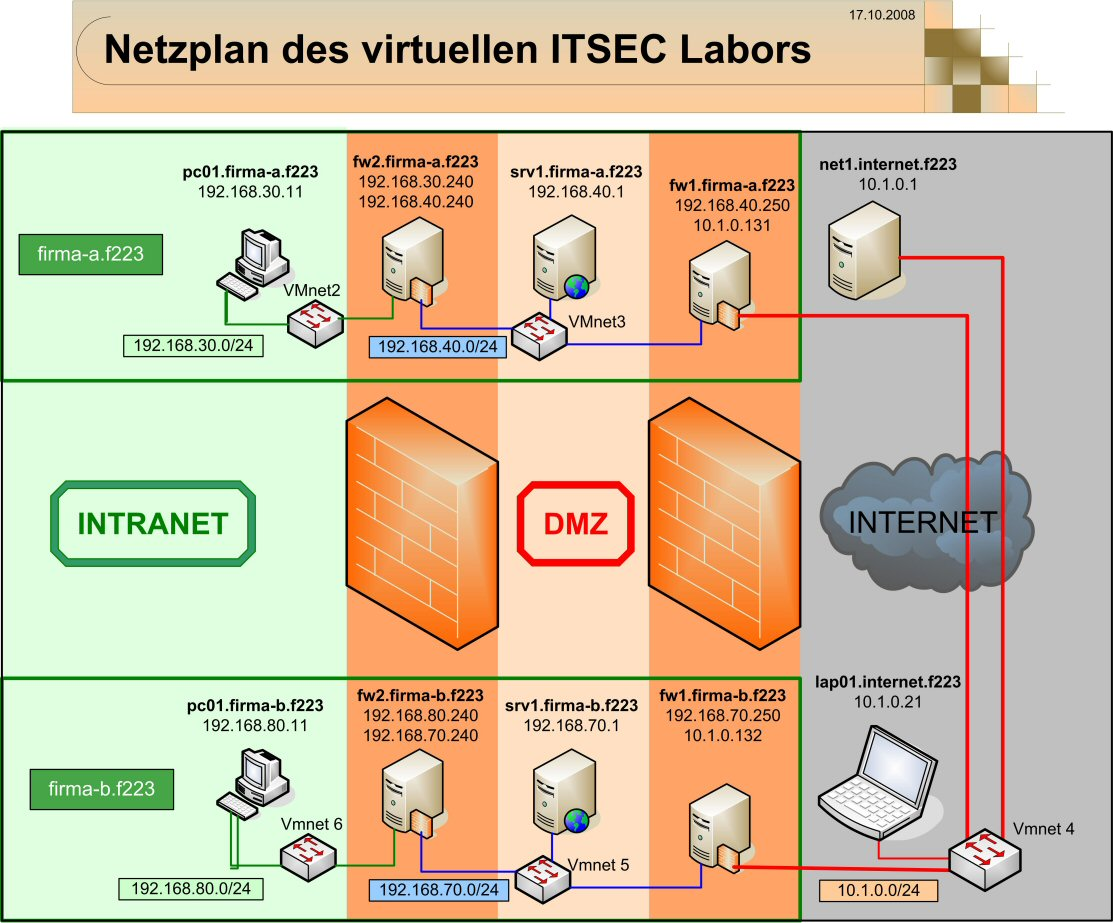
\includegraphics[width=0.9\textwidth]{figures/Netzplan.jpg}
  \caption{Netzplan des Versuchsaufbaus.\cite{labor}}
  \label{fig.netzplan}
\end{figure}

Dazu sind im Versuchsaufbau für jeden der in Abbildung 
\ref{fig.netzplan} abgebildeten Rechner
eine virtuelle Maschine bereitgestellt --- dies ermöglicht leichteres
Testen.

Wir haben uns dazu entschieden, das Netzwerk der \emph{Firma A} aufzubauen.
\emph{Firma B} bleibt unangetastet, und ist somit vollständig vorkonfiguriert,
was ebenfalls ein leichteres Testen ermöglicht, da der Web- und Mail-Server von
\emph{Firma B} aus dem "`Internet"' erreichbar ist und somit auch aus dem LAN
der \emph{Firma A} erreichbar sein muss.
Zudem lässt sich so der "`umgekehrte"' Fall testen: der Zugriff von einem
Rechner aus dem LAN von \emph{Firma B} auf die Dienste von
\emph{Firma A}.\cite{labor}


\newpage
\section{Linux Konfiguration}

Zunächst müssen zwei Debian 6.0 Maschinen,
mit der minimalen Installation, eingerichtet werden.
Diese repräsentieren die Firewallmaschinen {\tt fw1} und {\tt fw2} von
\emph{Firma A} aus Abbildung \ref{fig.netzplan}.
Zum Einrichten und Testen der Firewall-Rechner wurde noch weitere Software
installiert, welche in Kapitel \ref{sec.software} aufgelistet ist.
Die genaue Konfiguration der einzelnen Netzwerkadapter ist in Kapitel
\ref{sec.netzwerk} beschrieben.


\subsection{Software}\label{sec.software}

In der Debian-Installation sind die Befehle {\tt iptables} und {\tt route}
standardmäßig verfügbar.
Mit {\tt iptables} lassen sich IPv4-Pakete filtern und Network Address
Translations durchführen.
Der Befehl {\tt route} dient zum Ändern der IP-Routing-Tabellen des Kernels um
beispielsweise statische Routen für bestimmte Rechner oder Netzwerke
festzulegen.

Folgende zusätzliche Software wurde via {\tt apt-get}, Debians Paketmanager,
installiert:

\begin{itemize}
    \item iptstate --- IPTables State Top.\\
        Zeigt Informationen über die IP Tables state table an (siehe Kap.
        \ref{sec.tests}).
    \item resolvconf --- Nameserver information handler.\\
        Erlaubt es, die DNS-Nameserver in der Datei
        {\tt /etc/network/interfaces}
        per {\tt dns-nameservers 1.2.3.4 5.6.7.8} zu definieren und
        generiert daraus die benötigten Einträge in der {\tt /etc/resolv.conf}
        (siehe Listings \ref{lst:fw1:eth0} \& \ref{lst:fw2:eth1}).
    \item mcedit --- Internal file editor of GNU Midnight Commander.\\
        Text-Editor für die Konsole, welcher neben Aktionen wie Kopieren,
        Ausschneiden und Einfügen auch Syntax-Highlighting für eine Vielzahl von
        Dateitypen bietet. Hierfür muss der GNU Midnight Commander mittels des
        Pakets {\tt mc} installiert werden.
\end{itemize}


\subsection{Netzwerkadapter}\label{sec.netzwerk}

Die Netzweradapter wurden gemäß der in Abbildung \ref{fig.netzplan}
gezeigten IP-Adressen konfiguriert, dies geschieht über die Datei
{\tt /etc/network/interfaces}.

\subsubsection{\fwa}

Der Firewall Rechner {\tt fw1.firma-a.f223} befindet sich zwischen dem Extranet
(10.1.0.0/24) und der DMZ (192.168.40.0/24).
Damit ergibt sich für die beiden Netzwerkadapter folgende Konfiguration:

\paragraph{eth0} Verbindung zur DMZ.

\begin{lstlisting}[label=lst:fw1:eth0,caption={Netzwerkadapter eth0 Konfiguration.}]
allow-hotplug eth0
iface eth0 inet static
    address 192.168.40.250
    netmask 255.255.255.0
    broadcast 192.168.40.255
    dns-nameservers 192.168.40.1
    dns-search firma-a.f223
\end{lstlisting}

\paragraph{eth1} Verbindung zum Extranet bzw. Internet.

\begin{lstlisting}[label=lst:fw1:eth1,caption={Netzwerkadapter eth1 Konfiguration.}]
allow-hotplug eth1
iface eth1 inet static
    address 10.1.0.131
    netmask 255.255.255.0
    broadcast 10.1.0.0
\end{lstlisting}


\subsubsection{\fwb}

Die Konfiguration für den Firewall Rechner {\tt fw2.firma-a.f223}, der zwischen
der DMZ und dem Intranet (192.168.30.0/24) sitzt, sieht wie folgt aus:

\paragraph{eth0} Verbindung zum Intranet.

\begin{lstlisting}[label=lst:fw2:eth0,caption={Netzwerkadapter eth0 Konfiguration.}]
allow-hotplug eth0
iface eth0 inet static
    address 192.168.30.240
    netmask 255.255.255.0
    network 192.168.30.0
    broadcast 192.168.30.255
    dns-search firma-a.f223
\end{lstlisting}

\paragraph{eth1} Verbindung zur DMZ.

\begin{lstlisting}[label=lst:fw2:eth1,caption={Netzwerkadapter eth1 Konfiguration.}]
allow-hotplug eth1
iface eth1 inet static
    address 192.168.40.240
    netmask 255.255.255.0
    network 192.168.40.0
    broadcast 192.168.40.255
    dns-nameservers 192.168.40.1
\end{lstlisting}


\subsection{Nützliches}

\subsubsection{Einfacher Dateitransfer}

Um auf einfache Weise eine Datei von einem Rechner auf einen anderen zu
kopieren, ohne beispielsweise einen Telnet-, FTP- oder SSH-Server aufsetzen zu
müssen, bietet sich das Programm {\tt Netcat} an.
{\tt Netcat} erlaubt es als "`TCP/IP swiss army knife"'\footnote{
\url{http://nc110.sourceforge.net/}
} server- und client-seitig Daten von der Standardein- oder -ausgabe über
Netzwerkverbindungen zu transportieren.\\

\noindent Empfänger:
\begin{verbatim}
fw2 $ netcat -l -p 8080 > firewall-internal.sh
\end{verbatim}

\noindent Sender:
\begin{verbatim}
fw1 $ cat firewall-external.sh | netcat 192.168.40.240 8080
\end{verbatim}


\subsection{Bootskript}

Debian verwendet das von der Linux Standard Base spezifizierte
\emph{Init Script LSB}\footnote{
\url{http://wiki.debian.org/LSBInitScripts}}, welches Unterstützung
für \emph{dependency based boot sequencing}\footnote{
\url{http://wiki.debian.org/LSBInitScripts/DependencyBasedBoot}
} bietet. Das bedeutet, dass
die Programme die beim Aufstarten des Betriebssystems in einer idealen
Reihenfolge angeordnet werden, so dass es auch keine unangenehme Effekte
durch Abhängigkeiten der Programme untereinander entstehen.

Diese Bootskripte werden in {\tt /etc/init.d/} als Konfigurationsdateien
abgelegt und beginnen mit wohldefinierten Kopfzeilen, wie in Listing
\ref{lst:lsb-header} gezeigt.
In diesen Kopfzeilen kann neben einer Beschreibung auch das
Start- / Stopp-Verhalten sowie die Abhängigkeiten konfiguriert werden.

\begin{lstlisting}[label=lst:lsb-header,caption={Init Script LSB: Kopfzeilen.}]
### BEGIN INIT INFO
# Provides:          scriptname
# Required-Start:    $remote_fs $syslog
# Required-Stop:     $remote_fs $syslog
# Default-Start:     2 3 4 5
# Default-Stop:      0 1 6
# Short-Description: Start daemon at boot time
# Description:       Enable service provided by daemon.
### END INIT INFO
\end{lstlisting}

Die Angaben bei den Schlüsselwörtern {\tt Default-Start} und {\tt Default-Stop}
geben die Runlevel an, bei den das Skript gestartet beziehungsweise gestoppt
wird.
Für Debian Systeme sind die Runlevel laut Tabelle \ref{tab.runlevel} definiert.
\footnote{
\url{http://debiananwenderhandbuch.de/startstop.html}
}

\begin{table}[htb]
    \centering
    \begin{tabular}{|c|l|}
        \hline
        Runlevel & Beschreibung\\
        \hline
        0       & {\tt halt}, hält das System an, ohne es neu zu starten\\
        1       & Single-User Modus, minimal benötigte Dienste (Wartunsgarbeiten)\\
        2 bis 5 & Multiuser Modus, hier wird üblicherweise gearbeitet\\
        6       & {\tt reboot}, startet das System neu\\
        S und s & bringen das System in den Single-User Modus\\
        \hline
    \end{tabular}
   \caption{Runlevel bei Debian.}\label{tab.runlevel}
\end{table}

\noindent Im Normalbetrieb läuft ein Debian System im Runlevel 2.
Die zusätzlichen Multiuser Runlevel geben die Möglichkeit, verschiedene
Konfigurationen von Diensten einzurichten und den gewünschten Runlevel beim
Starten des Betriebssystems per Kernel-Parameter anzugeben.
Die Firewall-Skripte werden in allen Multiuser Modi gestartet und beim
Herunterfahren des Systems sowie im Single-User Modus, in dem keine
Netzwerkschnittstellen aktiv sind, gestoppt.

{\tt Required-Start} und {\tt Required-Stop} definieren die Dienste, die bei
der Aus\-füh\-rung des Skriptes bereits laufen oder noch laufen müssen.
Für die Firewall-Skripte haben wir an dieser Stelle
\verb!$local_fs $remote_fs $syslog $network! gewählt, da so das Netzwerk und
alle Dateisysteme vorhanden sind und auch der Syslog-Daemon eventuell
auftretende Fehler protokollieren kann.

Das Programm {\tt insserv}\footnote{
\emph{Vor} Debian 6.0 wird {\tt update-rc.d} verwendet.
} aktiviert installierte Init-Skripte, in dem es die passenden symbolischen
Links in den Runlevel-Verzeichnissen ({\tt /etc/init.d/rcX.d}) setzt:

\begin{verbatim}
insserv my_init_script
\end{verbatim}

Nach den Kopfzeilen kommt das eigentliche Skript, welches z.B. mittels
{\tt iptables} die Firewall konfiguriert, aber auch beliebige andere Programme
und Dienste können somit gestartet werden.

\begin{lstlisting}[label=lst:lsb-script,caption={Init Script LSB: Eigentliches Skript.}]
case "$1" in
    start)
        # Startup stuff
        echo "Daemon started."
        ;;
    stop)
        # Shutdown this service
        echo "Daemon stopped."
        ;;
    restart)
        # Restart this service
        echo "Daemon restarted."
        ;;
    *)
        # The default case
        echo "Usage $0 {start|stop|restart}"
        ;;
esac
\end{lstlisting}


\newpage
\section{Anforderungen}

Folgende Anforderungen für das Firewall-Konzept ergeben sich aus der
Aufgabenstellung:

\begin{itemize}
\item Mitarbeiter haben Zugang zum Internet.
      Die Arbeitsplatzrechner befinden sich im internen Netzwerk.
\item Die Website und der Mailserver der Firma soll vom Internet
      aus erreichbar sein.
      Dafür werden die Protokolle HTTP, HTTPS, SMTP und IMAP verwendet.
\item Einrichten einer multiplen DMZ,
      welche Webserver und Mailserver enthält.
      Der Zugriff auf das Internet vom internen Netzwerk erfolgt über die DMZ.
\item Die Firewalls sollen unerlaubte Zugriffe auf die DMZ und
      das Firmen-LAN verhindern.
\item Ein VPN-Zugriff auf das interne Netzwerk soll möglich sein.
      Dabei sollen sowohl die Netzwerke der beiden Unternehmen via LAN-to-LAN
      VPN gekoppelt werden können, als auch eine Einwahl der Mitarbeiter
      aus dem Internet ins interne Netzwerk der Firma möglich sein
      (Client-to-LAN).
\item Die Firma besitzt eine öffentliche IP-Adresse, darüber müssen die Dienste
      Webserver, Mailserver und VPN aus dem Internet erreichbar sein.
\item Die DNS-Server befinden sich auf {\tt srv1} (Firmenintern) und
      auf {\tt net1} (Internet).
\end{itemize}

\subsection{\fwa}

Um diesen Anforderungen gerecht zu werden
muss {\tt fw1} Connection Tracking verwenden.
Dabei werden Pakete, die zu einer bestehenden Verbindung gehören, akzeptiert.
Somit müssen nur Pakete, welche eine neue Verbindung aufbauen speziell betrachtet
werden. Es findet also eine Filterung der eingehenden Pakete statt, um DMZ und internes Netzwerk (LAN) zu schützen.
Desweiteren sind folgende Punkte umzusetzen:

\paragraph{§ 1 Zugriff auf das Internet}
\begin{itemize}
\item NAT und Masquerading: Pakete,
      die aus dem internen Netzwerk oder der DMZ ins Internet gehen,
      enthalten als Quelladresse nur die öffentliche IP-Adresse der externen
      Firewall (10.1.0.131).
\item Diese Pakte müssen auch entsprechend geroutet werden.
      (Forwarding- und Routing-Regeln)
\end{itemize}

\paragraph{§ 2 Mail- und Webserver}
\begin{itemize}
\item Eingehende Pakete an die entsprechenden Ports der öffentlichen IP-Adresse werden an {\tt srv1} weitergeleitet.
\item Dafür ist eine DNAT-Regel notwenig.
\item Protokolle: HTTP (80), HTTPS (443), SMTP (25, 465), IMAP (143, 993).
\end{itemize}

\paragraph{§ 3 VPN}
\begin{itemize}
\item Der VPN-Server befindet sich auf {\tt fw2}.
\item Weiterleitung der aus dem Internet eingehenden Pakete erfolgt mittels DNAT auf die UDP-Ports 1194 und 1195.
\end{itemize}

\paragraph{§ 4 DNS}
\begin{itemize}
\item Die Arbeitsplatzrechner im LAN verwenden {\tt srv1} für DNS-Anfragen.
\item Zur Auflösung von Hostnamen aus dem Internet (zB. www.firma-b.f223), muss {\tt srv1} die DNS-Anfragen an {\tt net1} weiterleiten können.
\item {\tt fw1} macht Forwarding der DNS-Pakete von {\tt srv1} zum Extranet.
\end{itemize}

\subsection{\fwb}

Um diesen Anforderungen gerecht zu werden
muss {\tt fw2} ebenfalls Connection Track\-ing verwenden.
Hauptaufgabe der {\tt fw2} ist der Schutz der Rechner im internen Netzwerk
der Firma.

\paragraph{§ 1 Zugriff auf das Internet}
\begin{itemize}
\item Mitarbeiter erhalten Zugriff auf das Internet.
\item Ausgehende Pakete aus dem LAN in Richtung des Extranets werden erlaubt.
\end{itemize}

\paragraph{§ 2 Mail- und Webserver}
\begin{itemize}
\item Mail- und Webserver sollen auch aus dem internen Netzwer erreichbar sein.
\item Forwarding der Pakete an Mail- und Webserver.
\end{itemize}

\paragraph{§ 3 VPN}
\begin{itemize}
\item Der VPN-Server läuft auf diesem Firewall Rechner.
\item Dafür müssen eingehende Pakete an die UDP-Ports 1194 und 1195 erlaubt werden.
\item Verwendung von virtuellen Netzwerkgeräten:
  \begin{itemize}
  \item LAN-to-LAN:\\
        Verwendung des Routing Modus von OpenVPN mittels TUN-Device,
        welches ein Point-to-Point-Netzwerkgerät simuliert und per IP-Paketen
        kommuniziert.
  \item Client-to-LAN:\\
        Verwendung des Bridging Modus von OpenVPN mittels TAP-Device,
        welches ein Ethernet-Gerät simuliert und über Ethernet-Frames
        kommuniziert.
  \end{itemize}
\item Der TUN- und der TAP-Adapter müssen jeweils bidirektional mit dem LAN kommunizieren können.
\end{itemize}

\paragraph{§ 4 DNS}
\begin{itemize}
\item Die DNS-Anfragen der Arbeitsplatzrechner müssen an {\tt srv1} weitergeleitet werden.
\end{itemize}


% \begin{appendix}
%   \include{chapters/a-setup}
% \end{appendix}

\addcontentsline{toc}{section}{Literaturverzeichnis}
\bibliographystyle{apalike}  % apalike
\bibliography{bib/references}

%\listoffigures
%\listoftables

\end{document}

